\section{Results} \label{sec:results}
\subsection{RQ1: Can we quantify interest of technical debt at the method-level?}
\smallsection{Motivation}
To alleviate the impact of technical debt, there are several previous studies on understanding SATD (e.g., the detection of technical debt~\cite{Potdar2014ICSME,Zazworka2013EASE} and the impact of SATD on software quality~\cite{Wehaibi2016SANER}).
However, there are few empirical studies that quantify interest of SATD.
Therefore, we would like to know how we can understand interest using our method explained in Section \ref{subsec:interest}

\smallsection{Approach}
%\para{We calculate the interest.}
To calculate interest of SATD, we follow the approach we explained in Section \ref{sec:setup}.

\smallsection{Results}
We find that there are high correlations between LOC and the other product metrics except Fan-In. 
From the highly correlated metrics, we choose LOC as metrics to calculate interest, similar to previous work that considers effort in the domain of defect prediction~\cite{Kamei2010ICSM,Kamei2013TSE}. We assume that developers spend more effort to check larger methods before modifying the methods. Eventually, we show our results using two product metrics (i.e., LOC and Fan-In).

Table \ref{tab:statistic} shows the number of SATD and the percentage of the technical debt that has positive interest in all technical debt. The table shows that 32.6\%-44.2\% of technical debt has a positve rate in terms of LOC and 30.9\%-42.2\% of technical debt has it in terms of Fan-In. 
There is not large difference of the positive rates between LOC and Fan-In. 
% The positive rate of LOC in ANT is 38.0% 

Figure \ref{fig:dist} shows that the distribution of interest for the technical debt of positive rate. The distribution in all plots are left-skewed (around 0 to 10). We can also find that some of positive intrest are over 100, which means the value of metric relatively increases by 100\%.
This findings suggest that we  have the technical debt that we preferentially allocate development research to solve.

\begin{table}[tb]
  \caption{Statistic interest of SATD}
  \label{tab:statistic}
  \centering

  \begin{tabular}{cl|r|rrr}
  \hline
      &  Project & Positive Rate & All & Positive & Negative \\
  \hline
        & Ant    & 38.0\% &  71 &  27  &  20 \\
   LOC  & JMeter & 44.2\% & 181 &  80  &  25 \\
        & JRuby  & 32.6\% & 236 &  77  &  59 \\
  \hline
        & Ant    & 30.9\% &  68 &  21  &  13 \\
Fan-In  & JMeter & 42.2\% & 161 &  68  &  13 \\
        & JRuby  & 30.3\% & 231 &  70  &  37 \\
  \hline
  \end{tabular}
\end{table}

%-----------------------------------------------------------------------
\begin{figure*}[!t]
  \begin{center}
  \scalebox{0.95}{
  \begin{tabular}{ccc}
    \subfigure[Ant (LOC)]{ 
      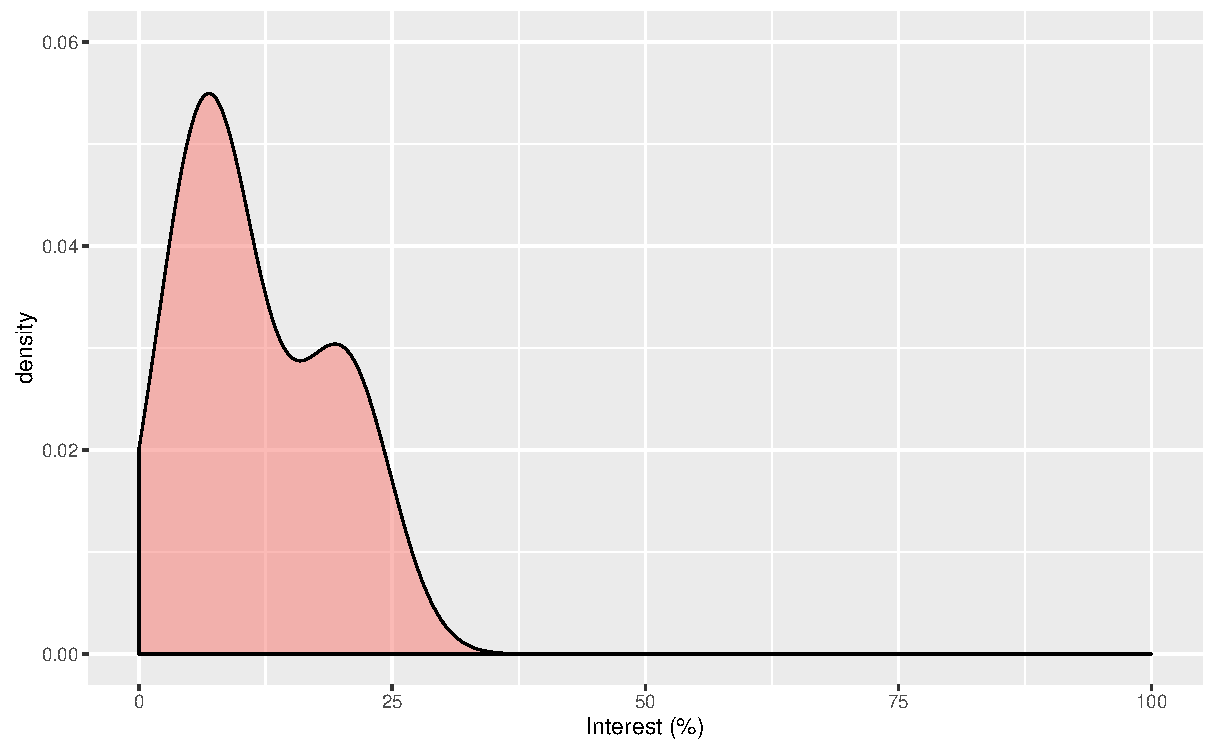
\includegraphics[width=.33\textwidth]{figures/rq1-ant}
    }
    \subfigure[JMeter (LOC)]{ 
      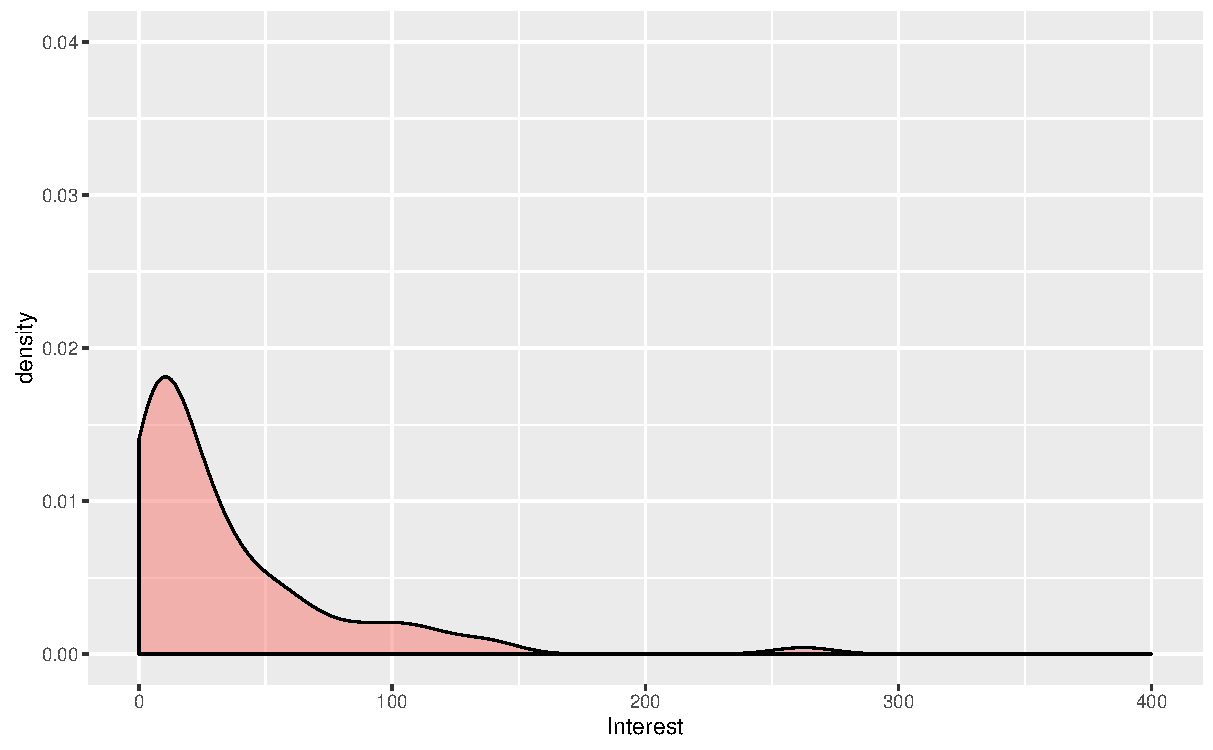
\includegraphics[width=.33\textwidth]{figures/rq1-jmeter}
    }
    \subfigure[JRuby (LOC)]{
      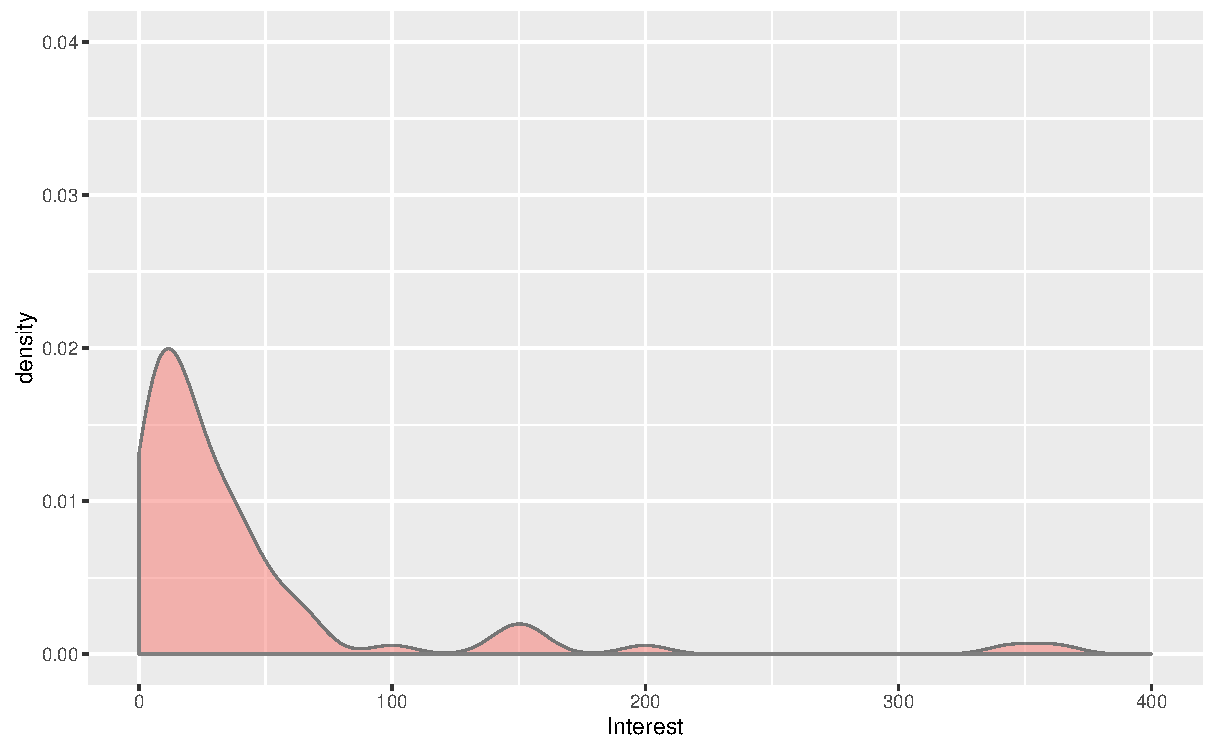
\includegraphics[width=.33\textwidth]{figures/rq1-jruby}
    }
  \end{tabular}
  }
  \scalebox{0.95}{
  \begin{tabular}{ccc}
    \subfigure[Ant (Fan-In)]{ 
      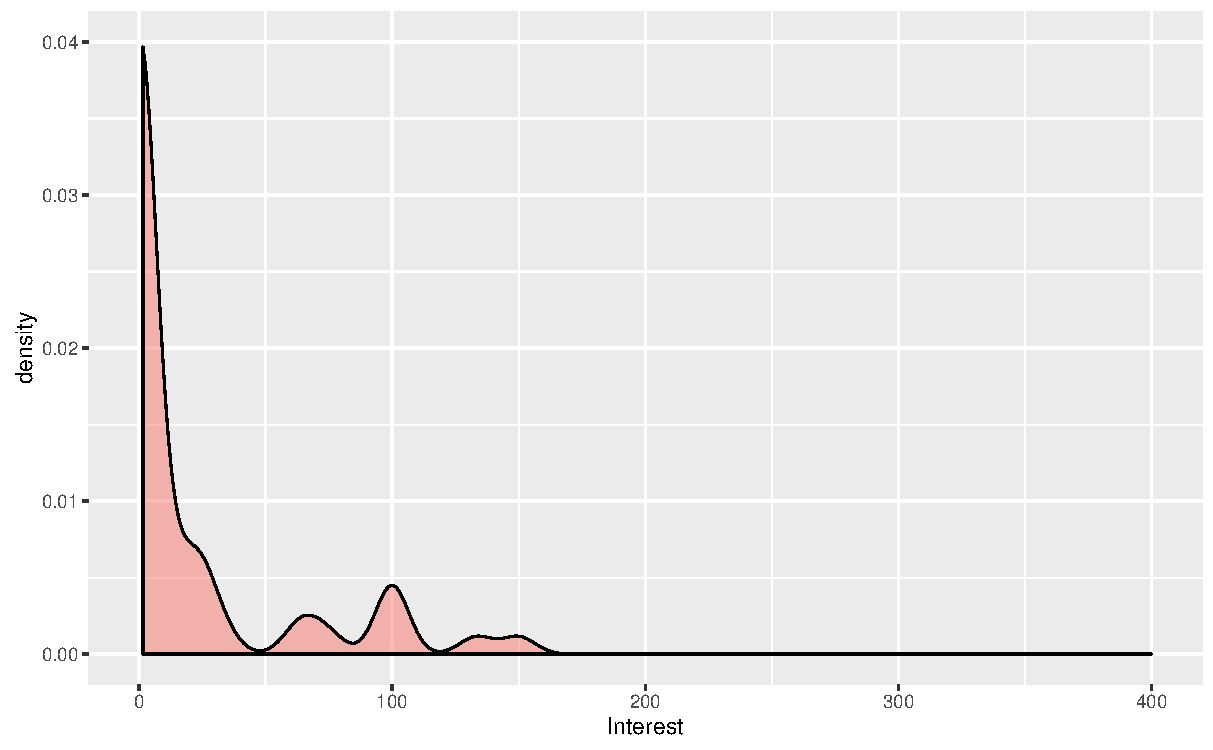
\includegraphics[width=.33\textwidth]{figures/rq1-ant-fanin}
    }
    \subfigure[JMeter (Fan-In)]{ 
      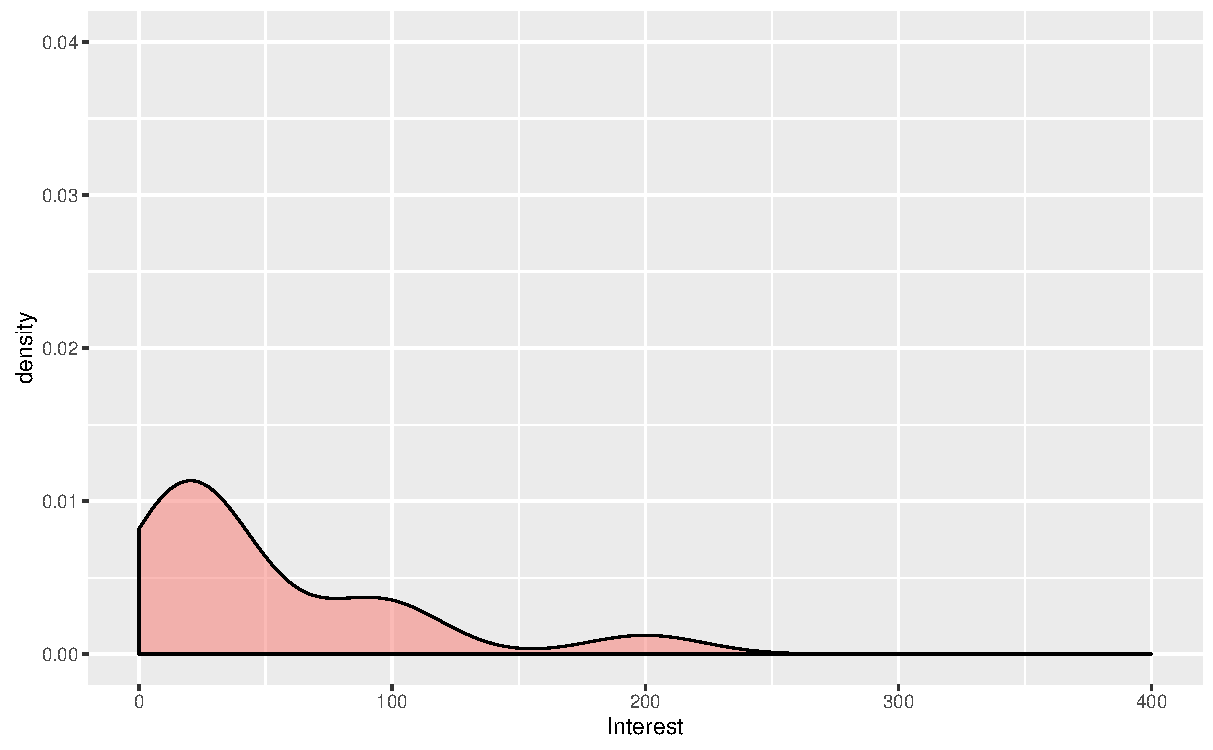
\includegraphics[width=.33\textwidth]{figures/rq1-jmeter-fanin}
    }
    \subfigure[JRuby (Fan-In)]{
      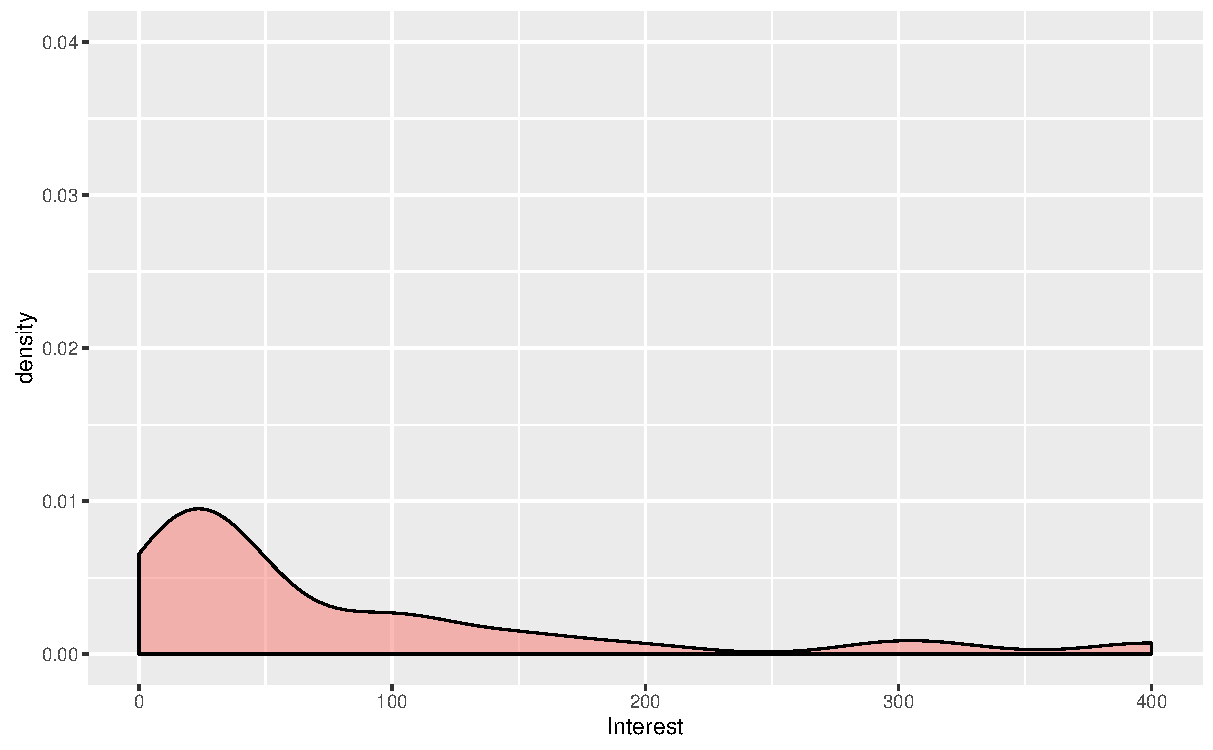
\includegraphics[width=.33\textwidth]{figures/rq1-jruby-fanin}
    }
  \end{tabular}
  }
  \caption{(RQ1) The results of distribution of interest.}
  \label{fig:dist}
  \end{center}
\end{figure*}
%-----------------------------------------------------------------------


\conclusionbox{
32.6\%-44.2\% of technical debt has a positive rate in terms of LOC and 30.9\%-42.2\% of technical debt has it in terms of Fan-In.}

\subsection{RQ2: Does the interest differ based on the type of technical debt?}
\smallsection{Motivation}
There are several type of technical debt such as defect technical debt and design technical debt.
The previous study~\cite{Maldonado2015MTD} shows that the percentage of technical debt varies depending on the type of technical debt and the studied systems. For example, the projects that have limited time to develop features are likely to leave comments of features that need to be implemented in the future. 
To better understand the interest, we would like to analyze the interest per type of technical debt.

\smallsection{Approach}
We classify technical debt into categories and calculate interest in each category.

\smallsection{Results}
Table X shows the number and the percentage of technical debt. Among three projects, jruby only includes more than one category that has more than 10\% of technical debt methods. Therefore, we decided to use jruby in RQ2.

\para{we report same things in RQ1.}  

\conclusionbox{Result of RQ2}

\subsection{RQ3: manual analysis}
\smallsection{Motivation}

\smallsection{Approach}

\smallsection{Results}

\conclusionbox{Result of RQ3}

%-----------------------------------------------------------------------
\begin{figure}
  \centering
  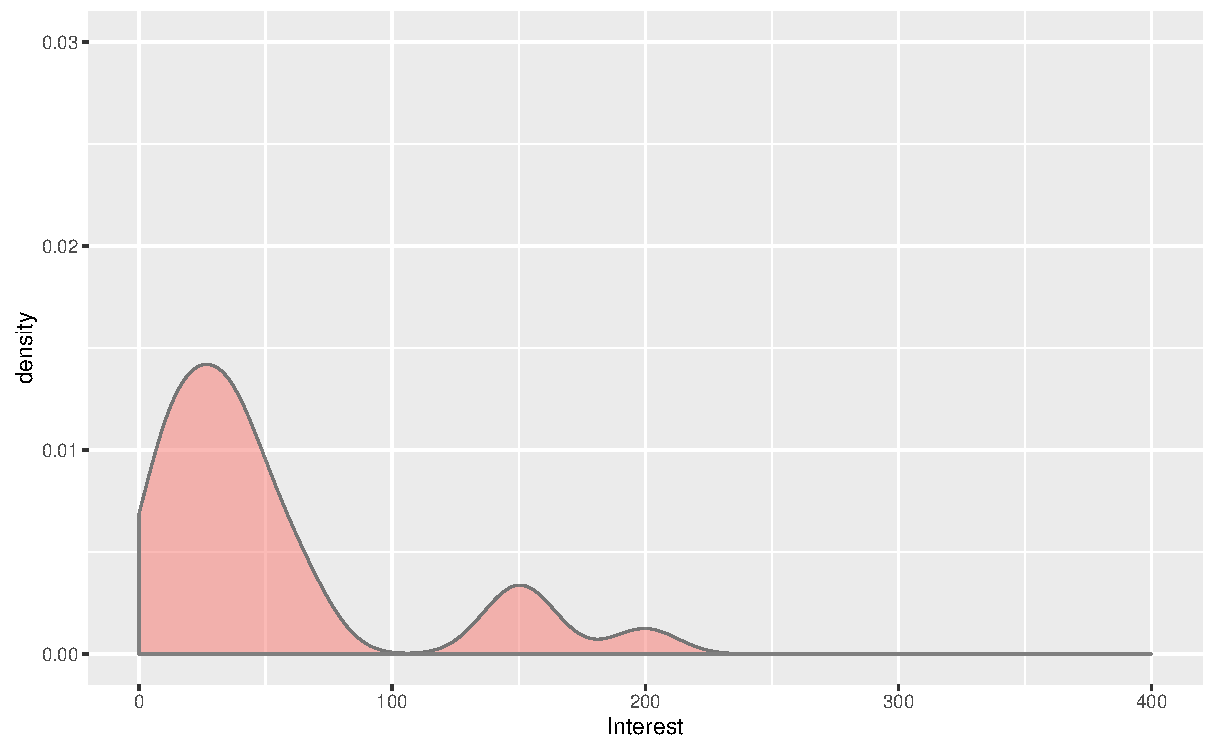
\includegraphics[width=.45\textwidth]{figures/rq2-defect}
  \caption{Adding a Repository in Commit Guru \label{fig:guru1}}
\end{figure}
\begin{figure}
  \centering
  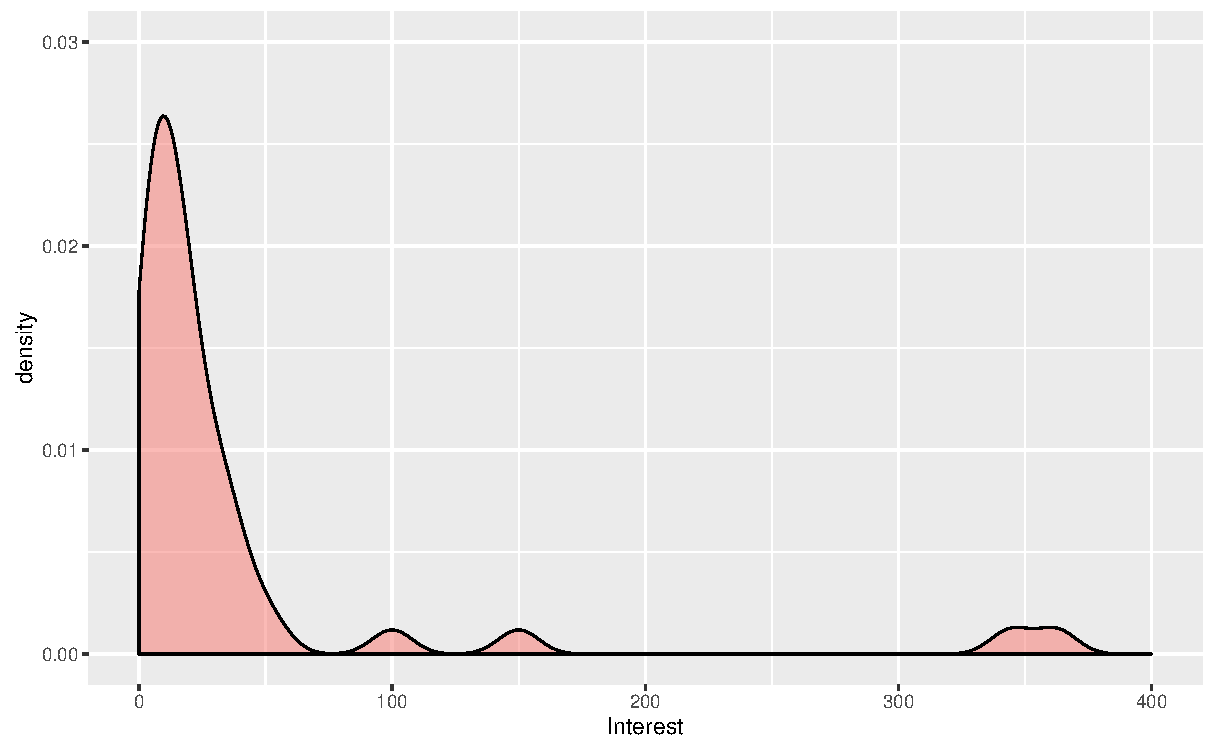
\includegraphics[width=.45\textwidth]{figures/rq2-design}
  \caption{Adding a Repository in Commit Guru \label{fig:guru1}}
\end{figure}
\begin{figure}
  \centering
  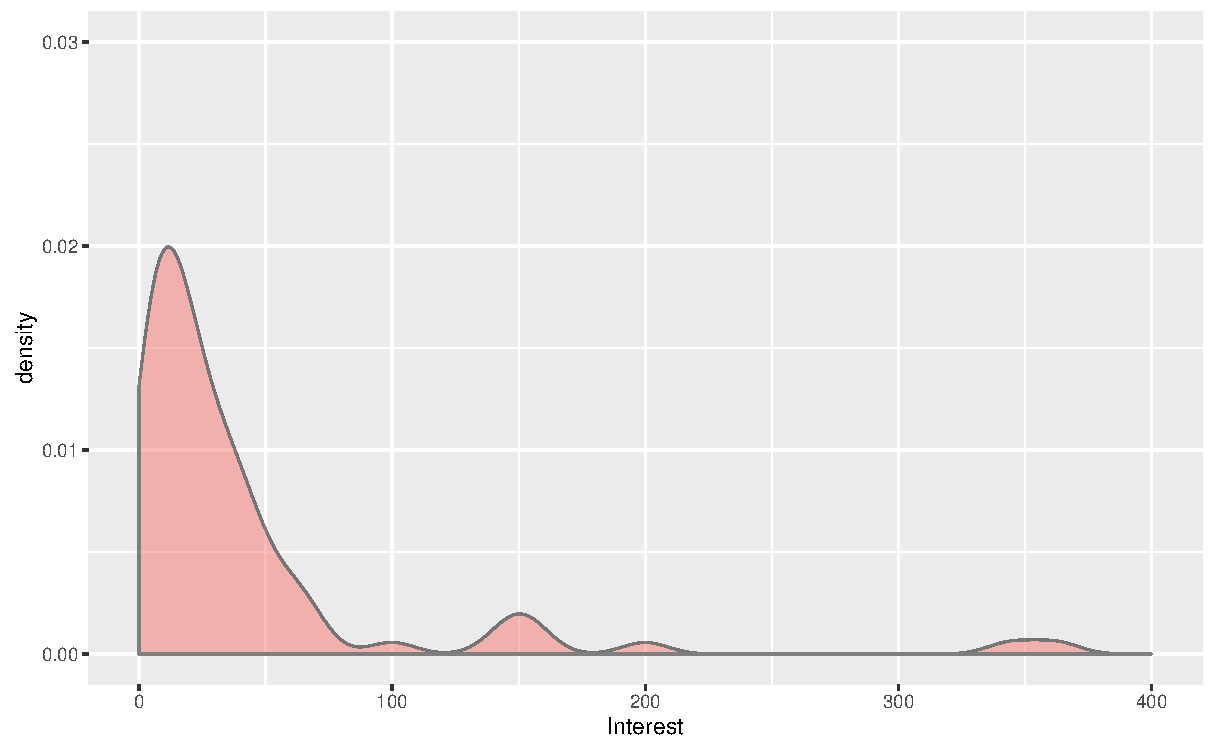
\includegraphics[width=.45\textwidth]{figures/rq2-requirement}
  \caption{Adding a Repository in Commit Guru \label{fig:guru1}}
\end{figure}
%-----------------------------------------------------------------------


\section{Discussion}
\para{Put additional analysis when considering time period.}

\para{Put additional analysis when considering other metrics (fan-in).}

%\para{Put additional analysis when comparing the non-technical deb methods.}
\smallsection{Motivation}
Generally speaking, software systems are always evolving over time for implementing new functionality and fixing defects~\cite{xxx}.
Therefore, even if the size of technical debt increases, it is not clear about how the nature of software evaluation affects the interest of technical debt.
We would like to compare the impact of software evolution on methods in two groups of SATD v.s. non-SATD.

\smallsection{Approach}
We compare the interest of methods between SATD and non-SATD.
We conduct the following steps:
\begin{itemize}
\item We obtain the list of files that include SATD.
\item We extract methods that do not include SATD.
\item We measure metrics for the methods in Step 2 at two versions that technical debt is introduced and removed.
\item We calculate interest using metrics in Step 3.
\end{itemize}
% What do we need to do some pre-condition for this analysis?

\smallsection{Result}

\para{Put the analysis for showing the method that includes more than one technical debt in one version.}